\documentclass[10pt]{article}

\usepackage{mathtools}  % need for math tools
\usepackage{amsmath}    % need for subequations
\usepackage{graphicx}   % need for figures
\usepackage{verbatim}   % useful for program listings
\usepackage{color}      % use if color is used in text
\usepackage{subfigure}  % use for side-by-side figures
\usepackage{hyperref}   % use for hypertext links, including those to external documents and URLs
\usepackage{graphicx}   % Used to import the graphics
\usepackage{subfig}     % Used to creat subfigs
\usepackage[version=3]{mhchem}     % Used to creat chemestry formula


\setlength{\baselineskip}{16.0pt}   
\setlength{\parskip}{3pt plus 2pt}
\setlength{\parindent}{20pt}
\setlength{\oddsidemargin}{0.5cm}
\setlength{\evensidemargin}{0.5cm}
\setlength{\marginparsep}{0.75cm}
\setlength{\marginparwidth}{2.5cm}
\setlength{\marginparpush}{1.0cm}
\setlength{\textwidth}{150mm}

\begin{document}

\begin{center}
{\large Ay190: Computational Astrophysics (Winter Term 2012)} \\
{\large HomeWork - 7 } \\
\copyright 2012 by Arya Farahi \\
Jan 27, 2012
\end{center}

\section{Exercise 1. pp-Chain Nucleosynthesis}


\bfseries{Part a : } \\ \mdseries

 $10^{20}$ would be a resonable end time for this problem. \\

\bfseries{Part b : } \\ \mdseries

\begin{figure}[hbt]
 \centering
 \label{fig:1} 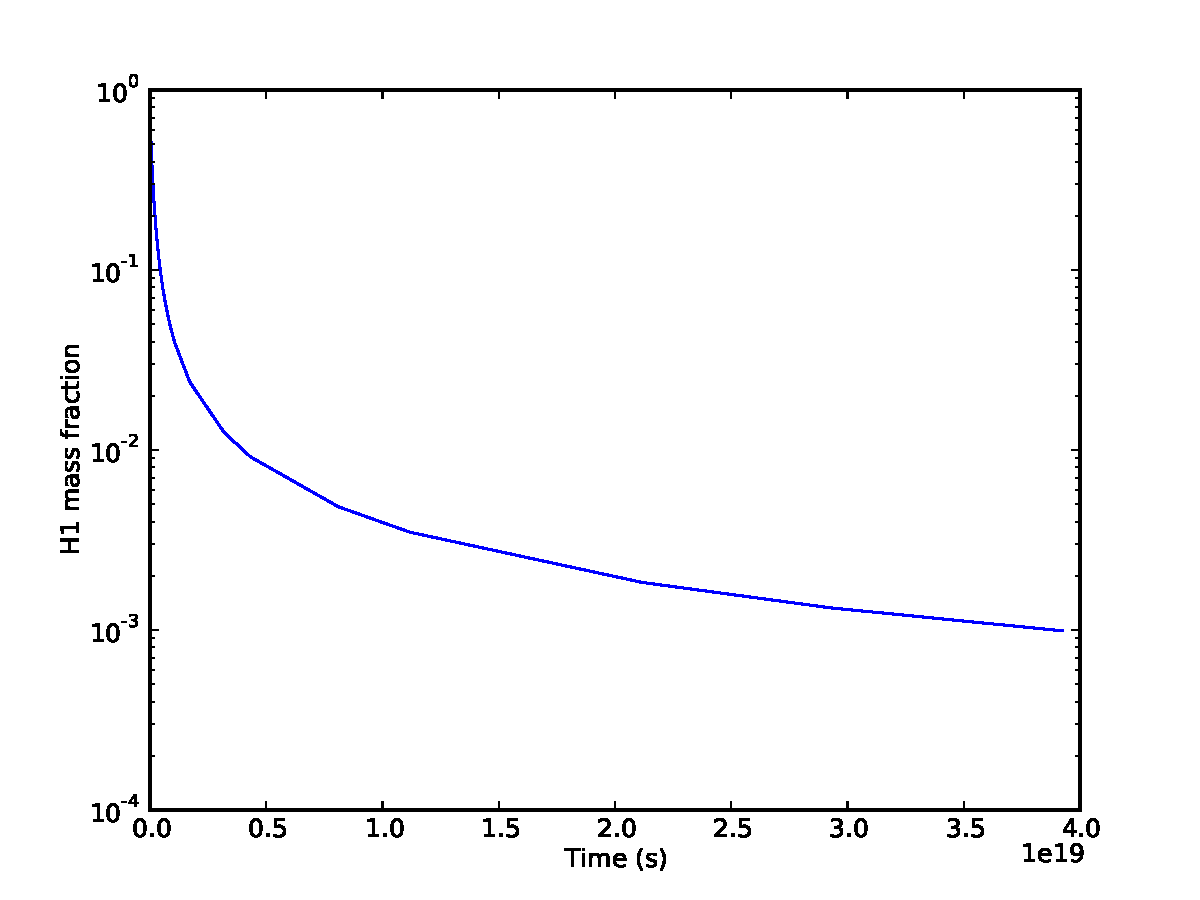
\includegraphics[scale=0.3]{Plots/plot1.pdf}
 \caption{ Plot of evolution of $^{1}\mathrm{H}$.}
\end{figure}

\begin{figure}[hbt]
 \centering
 \label{fig:2} 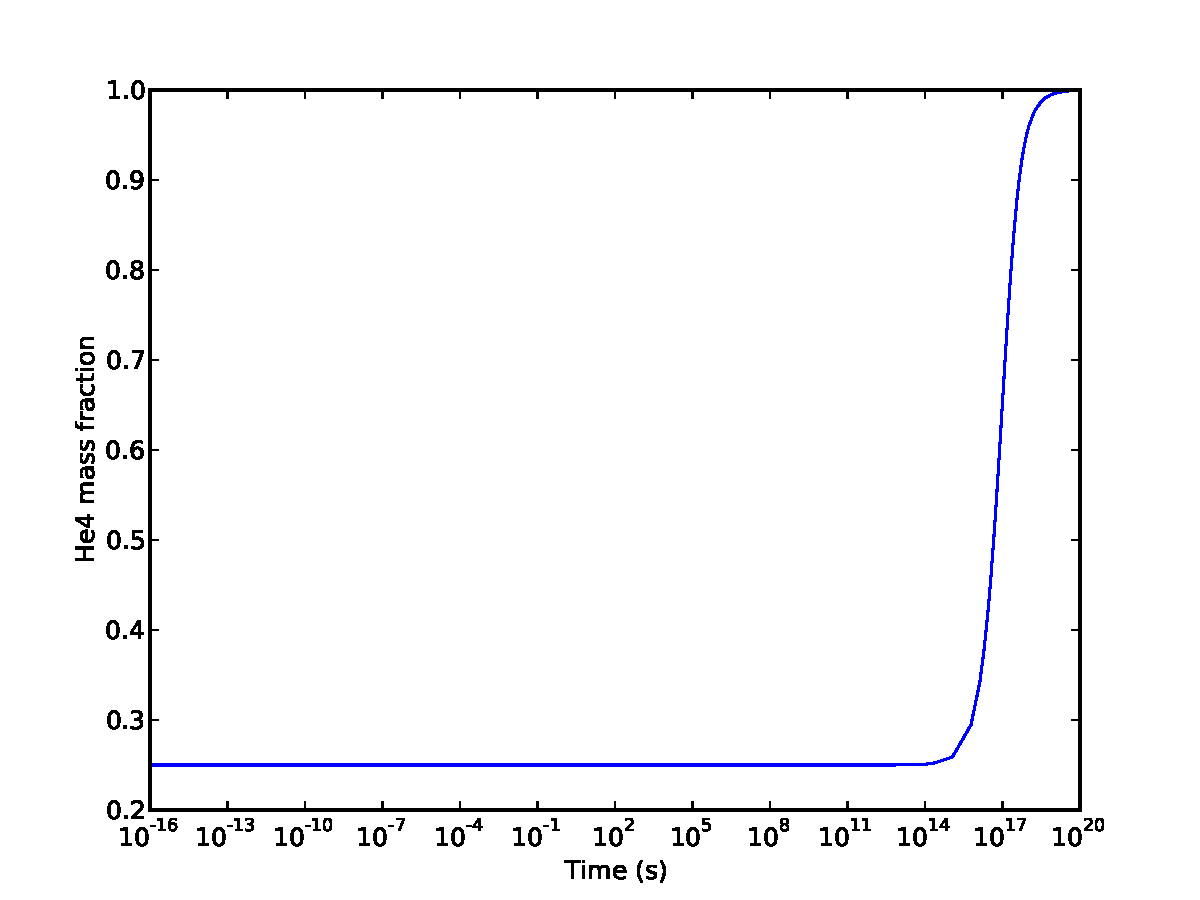
\includegraphics[scale=0.3]{Plots/plot2.pdf}
 \caption{ Plot of evolution of $^{4}\mathrm{He}$.}
\end{figure}

Figure \ref{fig:1} and \ref{fig:2} shows the evolution of $^{1}\mathrm{H}$ and $^{4}\mathrm{He}$ in semilogy and semilogx scale respectively.

\bfseries{Part c : } \\ \mdseries

When mass fraction of $^{1}\mathrm{H}$ is equal to: $0.000989$ then the mass fraction of $^{4}\mathrm{He}$ is equal to: $0.999$ at the center of the sun.


\bfseries{Part d : } \\ \mdseries

When mass fraction of $^{1}\mathrm{H}$ is equal to: $0.01$ then about $3.5^{18}$ (S) passed It means that sun burned for about $3.5^{18}$ (S)


\bfseries{Part e : } \\ \mdseries

The pp I branch \\

\ce{^{3}_{2}He + ^{3}_{2}He -> ^{7}_{4}Be + \gamma +} $12.86 \mathrm{MeV}$ \\

The pp II branch \\

\ce{^{3}_{2}He + ^{4}_{2}He -> ^{7}_{4}Be + \gamma } \\

\ce{^{7}_{4}Be + e^- -> ^{7}_{3}Li + \nu_e +} $0.861 \mathrm{MeV} / 0.383 \mathrm{MeV}$ \\

\ce{^{7}_{3}Be + ^{1}_{1}H -> 2 ^{4}_{2}He } \\
 
The pp III branch \\

\ce{^{3}_{2}He + ^{4}_{2}He -> ^{7}_{4}Be + \gamma } \\

\ce{^{7}_{3}Be + ^{1}_{1}H ->  ^{8}_{4}B + \gamma } \\

\ce{^{8}_{4}B             ->  ^{8}_{4}Be + e^+ + \nu_e + \gamma } \\

\ce{^{8}_{4}Be            -> 2 ^{4}_{2}He } \\

The pp IV (Hep) branch \\

\ce{^{3}_{2}He + ^{1}_{1}H -> ^{4}_{2}Be + e^+ + \nu_e +} $18.8 \mathrm{MeV}$ \\


\pagebreak




\end{document}
